\DiaryEntry{Catalan Numbers - Intro}{2022-06-15}{Combinatorics}

In combinatorial mathematics, the Catalan numbers are a sequence of natural numbers that occur in various counting problems, often involving recursively defined objects.

\subsection{Definition}

There is a recurrence relation for the Catalan numbers,

\be\label{2022-06-15:eq1}
C_{n+1} = \sum_{i=0}^n C_i C_{n-i}, \,\, n \geq 0, \quad C_0=1
\ee

from which we read off for the first Catalan numbers

\begin{align*}
  C_1 &= C_0 C_0 \\
  C_2 &= C_0 C_1 + C_1 C_0 \\
  C_3 &= C_0 C_2 + C_1 C_1 + C_2 C_0 \\
  C_4 &= C_0 C_3 + C_1 C_2 + C_2 C_1 + C_3 C_0 \\
  C_5 &= C_0 C_4 + C_1 C_3 + C_2 C_2 + C_3 C_1 + C_4 C_0
\end{align*}

In addition, the Catalan numbers can also be expressed directly as

\be\label{2022-06-15:eq2}
C_n = \frac{1}{n+1} {2n \choose n} = {2n \choose n} - {2n \choose n+1}
\ee

The first equation is handled further below, the second one can be ``seen'' by e.g. $n=4$:

\bee
{8 \choose 4} - {8 \choose 5} = \frac{8 \cdots 5}{1 \cdots 4} - \frac{8 \cdots 4}{1 \cdots 5} = \frac{8 \cdots 5 \cdot 5 - 8 \cdots 4 }{1 \cdots 5} =  \frac{8 \cdots 5}{1 \cdots 4} \frac{5-4}{5} = {8 \choose 4} \frac{1}{5} \qed
\eee

The first Catalan numbers are

\bee
    1, 1, 2, 5, 14, 42, 132, 429, 1430, 4862, 16796, 58786, \ldots
\eee

and they are sequence \href{https://oeis.org/A000108}{A000108} in the OEIS.

\subsection{Application, Proofs}

There are literally hundreds of things which the Catalan numbers count. See \cite{Stanley2015}. Here we concentrate on the ``main'' applications.

\paragraph{Counting Polygon Triangulations.} Let $\Pc_n$ denote a convex polygon with $n$ vertices. A triangulation of $\Pc_n$ is a set of $n-3$ diagonals which do not cross. A triangulation partitions the polygon $\Pc_{n+2}$ into $n$ triangles and we define the $n$th Catalan number as the number of triangulations of $\Pc_{n+2}$.

The triangulations for $\Pc_3, \Pc_4$ and $\Pc_5$ are shown in the following Figure.

\begin{figure}[H]
\centering
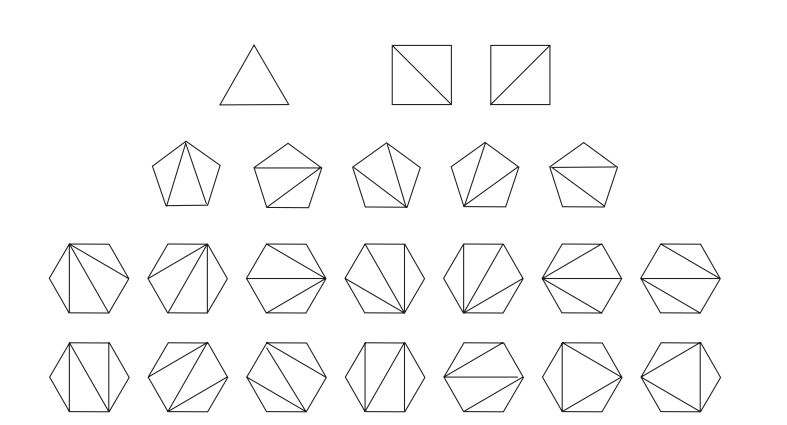
\includegraphics[scale=0.5]{images/2022-06-15-catalan_01.png}
\end{figure}

This counting argument allows to prove the recurrence relation \eqref{2022-06-15:eq1} as follows. Consider an $n+3$-polygon $\Pc_{n+3}$ (having $C_{n+1}$ triangulations). We can split this polygon into two polygons by removing an edge $e$ from $\Pc_{n+3}$. The resulting two polygons share one vertex and are denoted $\Qc_1$ and $\Qc_2$. They have $a_1+2$ and $a_2+2$ vertices, respectively. 

The following Figure shows an example of an $8$-polygon ($n=5$), having $C_6 = 132$ triangulations. The selected edge $e$ is shown in red; it splits the $8$-polygon into the $4$-polygon $\Qc_1$ with vertices $1,6,7,8$ ($a_1=2$) and the $5$-polygon $\Qc_2$ ($a_2=3$) with vertices $2,3,4,5,6$.

\begin{figure}[H]
\centering
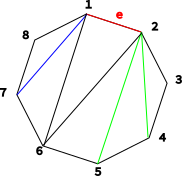
\includegraphics[scale=1.0]{images/2022-06-15-catalan_02.png}
\end{figure}

If we fix the edge $e$, $\Qc_1$ has $C_{a_1}= C_2=2$ different triangulations (one is shown in blue) and $\Qc_2$ has $C_{a_2}= C_3 = 5$ triangulations (one is shown in green). The ``additional'' edges due to creation of $\Qc_1$ and $\Qc_2$ (edges $1-6$ and $2-6$ in our example) also belong to the triangulation. These triangulations are ``independent''; i.e. we can fix one triangulation of $\Qc_1$ and choose one of the $C_{a_2}$ triangulations of $\Qc_2$. Therefore, the number of triangulations of $\Qc$ is $C_{a_1} C_{a_2}$ for a fixed edge $e$. We can choose the edge $e$ as any edge of the polygon, therefore the total number of triangulations of $\Pc_{n+3}$ is given by

\bee
C_{n+1} = \sum_{k=0}^n C_k C_{n-k} \qed
\eee

\paragraph{Counting Binary Trees.} A binary tree has a root vertex $v$, a left subtree $T_1$, and a right subtree $T_2$. The two subtrees are (again) binary trees. There are $C_n$ different binary trees with $n$ vertices. The following Figure shows the $C_3=5$ different binary trees with $n=3$ vertices.

\begin{figure}[H]
\centering

\includegraphics[scale=0.7]{images/2022-06-15-catalan_10.png}
\end{figure}


\paragraph{Counting Ballot Sequences.} A ballot sequence of length $2n$ is a sequence with $n$ $-1$s and $n$ $+1$s, such that every partial sum (i.e. the sum starts at the beginning) is non-negative. There are $C_n$ different ballot sequences of length $2n$. For $n=3$, we have the following $C_3=5$ ballot sequences,

\begin{align*}
  &+1, +1, +1, -1, -1, -1 \\
  &+1, +1, -1, +1, -1, -1 \\
  &+1, +1, -1, -1, +1, -1 \\
  &+1, -1, +1, +1, -1, -1 \\
  &+1, -1, +1, -1, +1, -1
\end{align*}


\paragraph{Counting Paranthesizations (or Bracketings).} Assume we have a string of $n+1$x's and a binary operation which we denote by $\cdot$. There are $C_n$ different ways to put parantheses on the string.

\begin{align*}
  &x \cdot (x\cdot (x\cdot x)) \\
  &x \cdot ((x\cdot x) \cdot x) \\
  &(x\cdot x)\cdot (x\cdot x) \\
  &(x \cdot ((x\cdot x))\cdot x \\
  &x((x\cdot x) \cdot x) \cdot x
\end{align*}

\paragraph{Counting Dyck Paths.} Finaly, we consider lattice paths on $\mZ^2$ from $(0,0)$ to $(2n,0)$ with steps $(1,1)$ and ($1,-1)$. A \emph{Dyck path} of length $2n$ is such a lattice path, wit the additional constraint that the path never passes below the $x$-axis.

Again, there are $C_n$ such Dyck paths of length $2n$. The following Figure shows the $5$ paths for $2n=6$.

\begin{figure}[H]
\centering
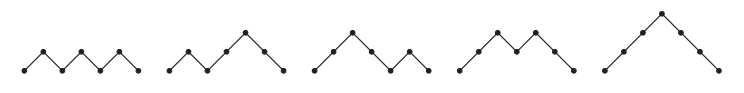
\includegraphics[scale=0.5]{images/2022-06-15-catalan_11.png}
\end{figure}

We can rotate the sheet and consider paths on $\mZ$ from $(0,0)$ to $(n,n)$ with steps $(1,0)$ and $(0,1)$. A Dyck path then goes from $(0,0)$ to $(n,n)$ but stays below the $y=x$ line. See the following Figure for an example.

\begin{figure}[H]
\centering
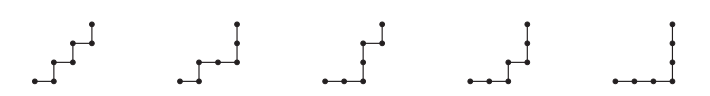
\includegraphics[scale=0.5]{images/2022-06-15-catalan_12.png}
\end{figure}

\subsection{Generating Function}

From the recurrence formulation \eqref{2022-06-15:eq1} we can derive the generating function. First we note that the binomial coefficient ${n \choose k}$ can be extended to real / complex $n$ by interpreting it as

\bee
{a \choose k} = \frac{a (a-1)(a-2) \cdots (a-k+1)}{k!}
\eee

with the understanding that the number of factors in denominator and numerator are the same. Using this, we get the ``generalized'' binomial theorem as

\bee
(1+x)^a = \sum_{n \geq 0} {a \choose k} x^n
\eee

for \emph{arbitrary} values of $a$; e.g. also real. As an example,

\begin{align*}
  \sqrt{1+x} &= \sum_{n \geq 0} {1/2 \choose k} x^n = {1/2 \choose 0} x^0 + {1/2 \choose 1} x^1 + {1/2 \choose 2} x^2 + {1/2 \choose 3} x^3 + \cdots \\
             &= 1 x^0 + \frac{1/2}{1}x + \frac{1/2 (-1/2)}{2!}x^2 + \frac{1/2 (-3/2) (-5/2)}{3!}x^3 + \cdots \\
             &= 1 + \frac{1}{2}x - \frac{1}{8}x^2 + \frac{1}{16}x^3 + \cdots \qed
\end{align*}

With that in place, we tackle the generating function $C(x)$ of the Catalan numbers. We start with

\bee
C_{n+1} = \sum_{i=0}^n C_i C_{n-i}, \,\, n \geq 0, \quad C_0=1
\eee

and multiply both sides by $x^n$ and sum over $n \geq 0$. On the left hand side we obtain

\bee
\sum_{n \geq 0} C_{n+1} x^n =  \frac{C(x) - C(0)}{x} = \frac{C(x) - 1}{x}
\eee

which comes from the (long forgotten :-) ) entry \ref{2015-09-07:entry}.  The right hand side is

\bee
\sum_{n \geq 0} x^n \left( \sum_{i=0}^n C_i C_{n-i} \right) = x^0 (C_0 C_0) + x^1 (C_0 C_1 + C_0 C_1) + x^2 (C_0 C_2 + C_1 C_1 + C_2 C_0) + \cdots
\eee

With some hindsight, let's consider $C^2(x)$ instead,

\begin{align*}
  C^2(x) &= (C_0 + C_1 x + C_2 x^2 + \cdots)^2 = C_0^2 + C_0 C_1 x + C_1 C_0 x + C_0 C_2 x^2 + C_1 C_1 x^2 + C_2 C_0 x^2 + \cdots \\
         &= C_0^2 + (C_0 C_1 + C_1 C_0)x + (C_0 C_2 + C_1 C_1 + C_2 C_0) x^2 \\
\end{align*}

and - surprisingly - this matches the right hand side of the recurrence equation. So we have

\bee
\frac{C(x) - 1}{x} = C^2(x)
\eee

which we can solve for the generating function as

\bee
C(x) = \frac{1 \pm \sqrt{1-4x}}{2x}
\eee

To determine the ``correct'' sign, we use Maxima

\begin{verbatim}
(%i2)	fp:(1 + sqrt(1-4*x))/(2*x);
(%o2)	(sqrt(1-4*x)+1)/(2*x)
(%i4)	taylor(fp, x, 0, 8);
(%o4)	1/x-1-x-2*x^2-5*x^3-14*x^4-42*x^5-132*x^6-429*x^7-1430*x^8+...
(%i5)	fm:(1 - sqrt(1-4*x))/(2*x);
(%o5)	(1-sqrt(1-4*x))/(2*x)
(%i6)	taylor(fm, x, 0, 8);
(%o6)	1+x+2*x^2+5*x^3+14*x^4+42*x^5+132*x^6+429*x^7+1430*x^8+...
\end{verbatim}

from which we deduce that the generating function of the Catalan numbers is

\bee
C(x) = \frac{1 - \sqrt{1-4x}}{2x} \qed
\eee

We can use the generating function to obtain the closed-form expressions \label{2022-06-15:eq2}: We use the series expansion of $\sqrt{1-4x}$,

\bee
\sqrt{1-4x} = \sum_{n \geq 0} {1/2 \choose n} (-4x)^n
\eee

in the generating function definition and obtain

\begin{align*}
  C(x) &= \frac{1}{2x} \left( 1 - \sum_{n \geq 0} {1/2 \choose n} (-4x)^n \right) \\
       &= \frac{1}{2x} - \frac{1}{2} \sum_{n \geq 0} {1/2 \choose n} (-4)^n x^{n-1} \\
       &= \frac{1}{2x} - \frac{1}{2} \left[ {1/2 \choose 0} \frac{1}{x} + {1/2 \choose 1} (-4)x^0 + {1/2 \choose 2} (-4)^2 x^1 + \cdots \right] \\
       &= -\frac{1}{2} \sum_{n \geq 1} {1/2 \choose n} (-4)^n x^{n-1} \\
       &= - \frac{1}{2} \sum_{n \geq 0} {1/2 \choose n+1} (-4)^{n+1} x^{n}
\end{align*}

from which we read off

\bee
C_n = -\frac{1}{2}  {1/2 \choose n+1} (-4)^{n+1}
\eee

Expanding this, we can somehow argue that this matches $C_n = \frac{1}{n+1} {2n \choose n}$. \todo{tidy this up...}

\bee
 -\frac{1}{2}  \frac{(1/2) (-1/2)(-3/2) \cdots }{(n+1)!} (-4)^{n+1} 
 \eee

 and the $4^{n+}$ kills off the $1/2$s in the numerator...

%%% Local Variables:
%%% mode: latex
%%% TeX-master: "journal"
%%% End:
